%	\author{Mitesh M. Khapra}
\title{Module 7}
\subtitle{Chapter 7: Beating humans at their own game (literally)}
\author{}
\institute{}
\date{}
%\institute{Department of Computer Science and Engineering\\ Indian Institute of Technology Madras}
%\titlegraphic{\includegraphics[height=1cm,width=2cm]{images/iitm_logo.png}}
%\titlegraphicii{\includegraphics[height=1cm,width=2cm]{logo2}}

\begin{frame}
	\myheading{Beating humans at their own game (literally)}
\end{frame}

\begin{frame}
	\begin{minipage}[t][0.6\textheight][t]{\textwidth}
		\begin{columns}
			\column{0.5\textwidth}
			\begin{overlayarea}{\textwidth}{\textheight}
				\justify
				\only<1>{\myheading{Playing Atari Games}}
				\only<2>{\myheading{Let's GO}}
				\only<3>{\myheading{Taking a shot at Poker}}
				\only<4>{\myheading{Defense of the Ancients}}
				\only<1>{\begin{itemize}
						\item{
						      Human-level control through deep reinforcement learning for playing Atari Games \cite{dqn}}
					\end{itemize}}
				\only<2>{\begin{itemize}
						\item{Alpha Go Zero - Best Go player ever, surpassing human players \cite{alphago}}
						\item{GO is more complex than chess because of number of possible moves}
						\item{No brute force backtracking unlike previous chess agents }
					\end{itemize}}
				\only<3>{\textbf{DeepStack} defeated 11 professional poker players with only one outside the margin of statistical significance \cite{deepstack}}
				\only<4>{\begin{itemize}
						\item{Widely popular game, with complex strategies, large visual space}
						\item{Bot was undefeated against many top professional players  }
					\end{itemize}}
			\end{overlayarea}
			\column{0.5\textwidth}
			\begin{overlayarea}{\textwidth}{\textheight}
				\begin{figure}
					\centering
					\only<1>{\includegraphics[scale=0.2]{images/module7/atari}}
					\only<2>{\includegraphics[scale=0.2]{images/module7/alphago}}
					\only<3>{\includegraphics[scale=0.15]{images/module7/poker}}
					\only<4>{\includegraphics[scale=0.15]{images/module7/dota}}
				\end{figure}
			\end{overlayarea}
		\end{columns}
	\end{minipage}
	\begin{minipage}[t][0.4\textheight][t]{\textwidth}
		\begin{overlayarea}{\textwidth}{\textheight}
			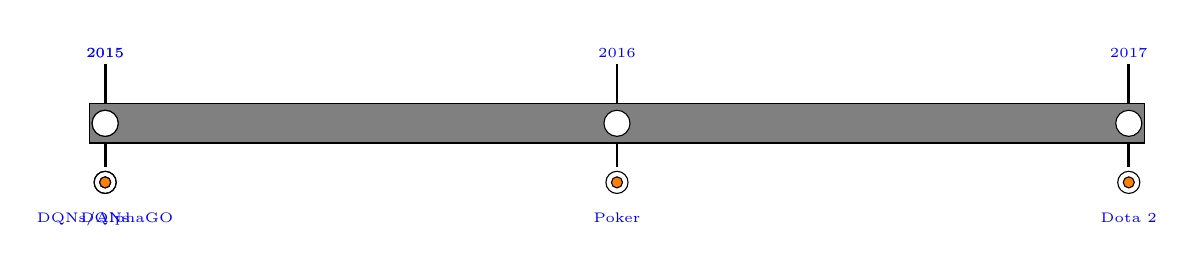
\begin{tikzpicture}[datemarker/.style={circle, draw=black,fill=white},textlabel/.style={anchor=center,text height=1.7ex,text depth=.25ex}]
				\tikzset{every node/.style={font=\tiny, color=blue}}\draw[fill=gray](-0.2,0) rectangle (13.2,0.5) node[white, below]{};
				\onslide<1->{\node at (0.0, 0.25) [datemarker] {};}
				\onslide<1->{\draw [line width=1pt] (0.0, 0.5) to (0.0, 1.0);}
				\onslide<1->{\draw (0.0, 1.2) node [textlabel]{2015};}
				\onslide<1->{\draw [fill=orange](0.0, -0.5) circle (2pt){};}
				\onslide<1->{\draw(0.0, -0.5) circle (4pt){};}
				\onslide<1->{\draw [line width=1pt] (0.0, 0) to (0.0, -0.3);}
				\onslide<1>{\draw (0.0,-0.9) node [textlabel] {DQNs};}
				\onslide<2->{\node at (0.0, 0.25) [datemarker] {};}
				\onslide<2->{\draw [line width=1pt] (0.0, 0.5) to (0.0, 1.0);}
				\onslide<2->{\draw (0.0, 1.2) node [textlabel]{2015};}
				\onslide<2->{\draw [fill=orange](0.0, -0.5) circle (2pt){};}
				\onslide<2->{\draw(0.0, -0.5) circle (4pt){};}
				\onslide<2->{\draw [line width=1pt] (0.0, 0) to (0.0, -0.3);}
				\onslide<2->{\draw (0.0,-0.9) node [textlabel] {DQNs/AlphaGO};}
				\onslide<3->{\node at (6.5, 0.25) [datemarker] {};}
				\onslide<3->{\draw [line width=1pt] (6.5, 0.5) to (6.5, 1.0);}
				\onslide<3->{\draw (6.5, 1.2) node [textlabel]{2016};}
				\onslide<3->{\draw [fill=orange](6.5, -0.5) circle (2pt){};}
				\onslide<3->{\draw(6.5, -0.5) circle (4pt){};}
				\onslide<3->{\draw [line width=1pt] (6.5, 0) to (6.5, -0.3);}
				\onslide<3->{\draw (6.5,-0.9) node [textlabel] {Poker};}
				\onslide<4->{\node at (13.0, 0.25) [datemarker] {};}
				\onslide<4->{\draw [line width=1pt] (13.0, 0.5) to (13.0, 1.0);}
				\onslide<4->{\draw (13.0, 1.2) node [textlabel]{2017};}
				\onslide<4->{\draw [fill=orange](13.0, -0.5) circle (2pt){};}
				\onslide<4->{\draw(13.0, -0.5) circle (4pt){};}
				\onslide<4->{\draw [line width=1pt] (13.0, 0) to (13.0, -0.3);}
				\onslide<4->{\draw (13.0,-0.9) node [textlabel] {Dota 2};}
			\end{tikzpicture}
		\end{overlayarea}
	\end{minipage}
\end{frame}
